%%%%%%%%%%%%%%%%%%%%%%%%%%%%%%%%%%%%%%%%%
% Masters/Doctoral Thesis 
% LaTeX Template
% Version 2.5 (27/8/17)
%
% This template was downloaded from:
% http://www.LaTeXTemplates.com
%
% Version 2.x major modifications by:
% Vel (vel@latextemplates.com)
%
% This template is based on a template by:
% Steve Gunn (http://users.ecs.soton.ac.uk/srg/softwaretools/document/templates/)
% Sunil Patel (http://www.sunilpatel.co.uk/thesis-template/)
%
% Template license:
% CC BY-NC-SA 3.0 (http://creativecommons.org/licenses/by-nc-sa/3.0/)
%
%%%%%%%%%%%%%%%%%%%%%%%%%%%%%%%%%%%%%%%%%

%----------------------------------------------------------------------------------------
%	PACKAGES AND OTHER DOCUMENT CONFIGURATIONS
%----------------------------------------------------------------------------------------
\documentclass[
11pt, % The default document font size, options: 10pt, 11pt, 12pt
%oneside, % Two side (alternating margins) for binding by default, uncomment to switch to one side
portuguese, % ngerman for German
singlespacing, % Single line spacing, alternatives: onehalfspacing or doublespacing
%draft, % Uncomment to enable draft mode (no pictures, no links, overfull hboxes indicated)
%nolistspacing, % If the document is onehalfspacing or doublespacing, uncomment this to set spacing in lists to single
%liststotoc, % Uncomment to add the list of figures/tables/etc to the table of contents
%toctotoc, % Uncomment to add the main table of contents to the table of contents
%parskip, % Uncomment to add space between paragraphs
%nohyperref, % Uncomment to not load the hyperref package
headsepline, % Uncomment to get a line under the header
chapterinoneline, % Uncomment to place the chapter title next to the number on one line
consistentlayout, % Uncomment to change the layout of the declaration, abstract and acknowledgements pages to match the default layout
]{MastersDoctoralThesis} % The class file specifying the document structure

\usepackage[utf8]{inputenc} % Required for inputting international characters
\usepackage[T1]{fontenc} % Output font encoding for international characters

\usepackage{mathpazo} % Use the Palatino font by default

\usepackage[autostyle=true]{csquotes} % Required to generate language-dependent quotes in the bibliography

\usepackage{subfigure}

\usepackage[backend=biber, style=numeric,]{biblatex}

\addbibresource{mendeley_v2.bib} % The filename of the bibliography

%----------------------------------------------------------------------------------------
%	MARGIN SETTINGS
%----------------------------------------------------------------------------------------

\geometry{
	paper=a4paper, % Change to letterpaper for US letter
	inner=2.5cm, % Inner margin
	outer=3.8cm, % Outer margin
	bindingoffset=.5cm, % Binding offset
	top=1.5cm, % Top margin
	bottom=1.5cm, % Bottom margin
	%showframe, % Uncomment to show how the type block is set on the page
}

%% make labels in bibliobraphy be #.
\makeatletter
\renewcommand\@biblabel[1]{#1.}
\makeatother   

%% make citations be superscripts, taken from citesupernumber.sty
\makeatletter
\def\@cite#1#2{$^{\mbox{\scriptsize #1\if@tempswa , #2\fi}}$}
\makeatother


%----------------------------------------------------------------------------------------
%	THESIS INFORMATION
%----------------------------------------------------------------------------------------

\thesistitle{Classificador supervisionado de atividades e comandos baseado em Variabilidade de Frequência Cardíaca} % Your thesis title, this is used in the title and abstract, print it elsewhere with \ttitle
\supervisor{Prof. Dr. André Fujita} % Your supervisor's name, this is used in the title page, print it elsewhere with \supname
\examiner{} % Your examiner's name, this is not currently used anywhere in the template, print it elsewhere with \examname
\degree{Master of Science} % Your degree name, this is used in the title page and abstract, print it elsewhere with \degreename
\author{Juliana Cavalcanti Correa} % Your name, this is used in the title page and abstract, print it elsewhere with \authorname
\addresses{} % Your address, this is not currently used anywhere in the template, print it elsewhere with \addressname

\subject{Bioinformática} % Your subject area, this is not currently used anywhere in the template, print it elsewhere with \subjectname
\keywords{} % Keywords for your thesis, this is not currently used anywhere in the template, print it elsewhere with \keywordnames
\university{Universidade de São Paulo} % Your university's name and URL, this is used in the title page and abstract, print it elsewhere with \univname
\department{Instituto de Matemática e Estatística} % Your department's name and URL, this is used in the title page and abstract, print it elsewhere with \deptname
\group{Programa de Pós-Graduação Interunidades em Bioinformática} % Your research group's name and URL, this is used in the title page, print it elsewhere with \groupname
\faculty{\href{http://faculty.university.com}{Faculty Name}} % Your faculty's name and URL, this is used in the title page and abstract, print it elsewhere with \facname

\AtBeginDocument{
\hypersetup{pdftitle=\ttitle} % Set the PDF's title to your title
\hypersetup{pdfauthor=\authorname} % Set the PDF's author to your name
\hypersetup{pdfkeywords=\keywordnames} % Set the PDF's keywords to your keywords
}

\begin{document}

\frontmatter % Use roman page numbering style (i, ii, iii, iv...) for the pre-content pages

\pagestyle{plain} % Default to the plain heading style until the thesis style is called for the body content

%----------------------------------------------------------------------------------------
%	TITLE PAGE
%----------------------------------------------------------------------------------------

\begin{titlepage}
\begin{center}

\vspace*{.06\textheight}
{\scshape\LARGE \univname\par}\vspace{1.5cm} % University name
\textsc{\Large Relatório para Exame de Qualificação}\\[0.5cm] % Thesis type

\HRule \\[0.4cm] % Horizontal line
{\huge \bfseries \ttitle\par}\vspace{0.4cm} % Thesis title
\HRule \\[1.5cm] % Horizontal line
 
\begin{minipage}[t]{0.4\textwidth}
\begin{flushleft} \large
\emph{Autor:}\\
\href{mailto:julicc@ime.usp.br}{\authorname} % Author name - remove the \href bracket to remove the link
\end{flushleft}
\end{minipage}
\begin{minipage}[t]{0.4\textwidth}
\begin{flushright} \large
\emph{Orientador:} \\
\href{mailto:fujita@ime.usp.br}{\supname} % Supervisor name - remove the \href bracket to remove the link  
\end{flushright}
\end{minipage}\\[3cm]
 
\vfill

%%\large \textit{A thesis submitted in fulfillment of the requirements\\ for the degree of \degreename}\\[0.3cm] % University requirement text
%%\textit{in the}\\[0.4cm]
\groupname\\\deptname\\[2cm] % Research group name and department name
 
\vfill

{\large \today}\\[4cm] % Date
%\includegraphics{Logo} % University/department logo - uncomment to place it
 
\vfill
\end{center}
\end{titlepage}

%----------------------------------------------------------------------------------------
%	ABSTRACT PAGE
%----------------------------------------------------------------------------------------

\begin{abstract}
Heart Rate Variability (HRV) is a measure of physiological state linked to the autonomous nervous system and its reactions to stress stimuli. In this work, we investigate the feasibility of using it as a biological marker of human activities and intentions. We propose a pipeline to extract and process HRV from the heart rate signal obtained from non-invasive chest straps, preparing its data to run through analysis and classifiers. We then derive one such classifier for human daily activities and propose biofeedback methods for a subject to increase or decrease his HRV, which would allow us detect his intention from the same features of the HRV signal that allowed us to build the classifier, thus developing a human-machine interaction that can, in some cases, be used in place of EEG-based methods, which rely on costly equipment.
\end{abstract}

\tableofcontents % Prints the main table of contents

%----------------------------------------------------------------------------------------
%	CONTENT - CHAPTERS
%----------------------------------------------------------------------------------------

\mainmatter % Begin numeric (1,2,3...) page numbering

\pagestyle{thesis} % Return the page headers back to the "thesis" style

\chapter{Introdução} 
\label{intro}

%----------------------------------------------------------------------------------------
%	Objetivos
%----------------------------------------------------------------------------------------

    \section{Objetivos}
    \label{goals}
    
        \paragraph{} A Variabilidade da Frequência Cardíaca (Heart Rate Variability - HRV) provê uma janela não-invasiva para funções do sistema nervoso autônomo e vem sendo amplamente utilizada por atletas para medição de aptidão física e recuperação de treinamento, e pela comunidade de saúde como uma medida da resposta involuntária ao estresse. Nosso principal objetivo nesse trabalho é explorar a informação contida nesse sinal e avaliar a viabilidade de seu uso em outras áreas, tais como seu potencial para ser utilizada em uma interface humano-máquina. 
        
        \paragraph{} A principal motivação para isso é o fato de que o sinal de HRV é de fácil obtenção, podendo ser coletado através de sensores com eletrodos ou até mesmo relógios de pulso que meçam os intervalos entre batimentos cardíacos com precisão. Isso lhe permitiria ser uma alternativa viável, em algumas circunstâncias, ao uso de equipamentos mais caros e desconfortáveis para obtenção de informação semelhante via EEG.
        
        \subsection{Pipeline para tratamento de dados para classificação de HRV}
        
            \paragraph{} Para poder explorar a informação contida no sinal de HRV, nosso primeiro objetivo é definir e implementar um pipeline que nos permita coletar o dado bruto de intervalos entre batimentos cardíacos, armazená-los em um banco de dados com anotações manuais com as quais possam ser relacionados e processá-los de forma a obter datasets completos que sirvam de entrada para classificadores. 
            \paragraph{} Desejamos que esse pipeline possa ser usado, primeiramente nos classificadores descritos a seguir, mas que seja flexível o suficiente para que possa servir de suporte a quaisquer pesquisas que visem a  explorar o dado de HRV em conjunto com alguma outra variável.
        
        \subsection{Classificação supervisionada de atividades}
        
            \paragraph{} O primeiro tipo de informação que buscamos no dado de HRV processado é sobre as atividades diárias de um indivíduo. Como o tipo de atividade exercida pode influenciar a frequência cardíaca, desejamos responder se é possível, e com que nível de granularidade, classificar as atividades realizadas por um indivíduo durante seu dia-a-dia usando apenas a informação da frequência cardíaca. Essa classificação poderia servir como dado de apoio para fornecer contexto a sistemas de detecção mais detalhados via EEG, a aplicações de \textit{lifelogging}, ou até mesmo para análise em tempo real de respostas involuntárias ao estresse externo.
       
        \subsection{Classificação supervisionada de manipulação de HRV - IHC}
            
            \paragraph{} Uma vez entendidos quais parâmetros permitem a classificação de atividades, nosso próximo objetivo é tentar elevar ou reduzir o HRV voluntariamente através de técnicas de \textit{biofeedback}, para replicar, controladamente, as alterações nesses parâmetros. Com isso, esperamos conseguir controlar uma Interface Humano-Máquina (IHC), mesmo que de maneira simples. Por ser não-invasivo e obtido através de sensor razoavelmente confortável e discreto, essa interface poderia ter aplicações em áreas que exigem, hoje, \textit{hardware} mais sofisticado e caro para essa interação.


%----------------------------------------------------------------------------------------
%	Revisão bibliográfica
%----------------------------------------------------------------------------------------

    \section{HRV}
    \label{HRV}
        
        \subsection {Definição e obtenção}
        \paragraph{} O coração saudável não tem um ritmo regular como o de um metrônomo. Seu ritmo sofre oscilações constantes e complexas, que permitem que o sistema cardiovascular se adapte rapidamente a alterações físicas e fisiológicas no ambiente ~\cite{Hansen2004HeartDetraining}. A Variabilidade da Frequência Cardíaca (HRV) é uma medida da variação dos intervalos entre batimentos consecutivos, chamados \textit{Interbeat Intervals} (IBI) ou intervalos RR. O nome de intervalo RR se deve ao fato de que esses intervalos são calculados como a distância entre dois picos do complexo QRS que é parte da forma de onda de um eletrocardiograma (ECG). ~\cite{TaskForceoftheEuropeanSocietyofCardiologytheNorthAmericanSocietyofPacing1996HeartUse}
        
        \paragraph{} A série de intervalos RR é derivada do próprio ECG, o qual mede os ciclos de polarização originados no nó sinoatrial, que fazem com que o átrio e o ventrículo se contraiam em ciclos, dando origem aos batimentos cardíacos. O ECG pode ser obtido em laboratório, com o uso de eletrodos, o \textit{gold-standard} do método, porém estudos \cite{Plews2017ComparisonMethods, Giles2016ValidityRest.} demonstram que algumas cintas torácicas disponíveis comercialmente com eletrodos embutidos, frequentemente utilizadas por atletas para medir seus treinamentos, têm precisão comparável à de um ECG em laboratório, viabilizando seu uso para projetos de pesquisa. 
        
        \paragraph{} Outro método para obter a frequência cardíaca e derivar o HRV é através da fotopletismografia (PPG), amplamente utilizada em \textit{smartwatches} disponíveis comercialmente e até em \textit{softwares} que usam uma câmera de celular posicionada sobre o dedo. Essa técnica mede a frequência cardíaca indiretamente, através da variação na absorção de luz verde pela pele ocasionada pela variação de fluxo sanguíneo. 
       
        \subsection {Regulação autonômica}
        
        \paragraph{} O nó sinoatrial, conhecido por ser o marcapasso natural do coração, gera aproximadamente 100 pulsos elétricos por minuto. No entanto, essa taxa não é regular, mas sim modulada por sinais oriundos do Sistema Nervoso Autônomo (SNA), o qual é composto por dois ramos opostos. 
        
        O Sistema Nervoso Simpático (SNS) é responsável por reações a estímulos externos de estresse, desencadeando reações tais como o aumento da frequência cardíaca e do fluxo sanguíneo e a dilatação das pupilas. Ele é responsável por deixar o corpo pronto para reagir ao estímulo. 
        
        O Sistema Nervoso Parassimpático, por sua vez, age como um freio a esse sistema quando não há estímulo externo, permitindo que o organismo relaxe, reduza a frequência cardíaca e a pressão sanguínea e retome as atividades normais ~\cite{Oweis2014QRSSurvey}. Ele também é responsável por manter o ritmo regular da respiração e seu principal componente, o nervo vago, tem papel crucial nos mecanismos de digestão e regulação da homeostase. A ação concorrente desses dois sistemas cria as flutuações sutis nos intervalos detectadas pelos métodos de análise de HRV.
      
        \subsection {Usos na literatura}
        
            \paragraph{} A primeira descrição do HRV foi no contexto de um método não-invasivo de  deteção de angústia fetal. Todavia, ele foi, desde então, adotado amplamente nas áreas de saúde e esporte ~\cite{Quintana2016GuidelinesCommunication}. 
            
            Na medicina esportiva, é usado para monitorar a recuperação de atletas, indicando quando estão ou não aptos a realizar treinos mais pesados, o que reduz a probabilidade de lesões. ~\cite{Oweis2014QRSSurvey, Plews2017ComparisonMethods, Shaffer2017AnNorms.}. 
            
            Por outro lado, em estudos das áreas de psicologia e psiquiatria, o HRV é considerado um marcador de estresse ~\cite{ Bernardi2000EffectsVariability, Castaldo2015AcuteMeta-analysis, Prinsloo2011TheStress, Vanitha2014HierarchicalVariability,}, bem como é usado em técnicas de \textit{biofeedback} que tentam regular o estresse ~\cite{Sasaki2014ConsciouslyActivity} e até mesmo como indicador de comorbidades psiquiátricas ~\cite{Quintana2016GuidelinesCommunication}. Em particular, em ~\cite{Salahuddin2007UltraSettings}, os autores demonstram que é possível encontrar marcadores de estresse nos parâmetros de HRV em intervalos curtos, a partir de 30 segundos.
            
            \paragraph{} Pesquisas também sugerem que o HRV é importante para o funcionamento efetivo em tarefas complexas, impactando diretamente o funcionamento do córtex pré-frontal ~\cite{Hansen2004HeartDetraining, Prinsloo2011TheStress, Luque-Casado2013CognitiveLevel}. Em  ~\cite{Hansen2004HeartDetraining}, os autores mostram que a performance em testes cognitivos é correlacionada com a atividade parassimpática, medida pela potência do espectro de alta frequência, e que, por sua vez, essa é correlacionada com o treinamento físico.
            
            \paragraph{} Estudos anteriores obtiveram sucesso aplicando classificadores sobre séries de intervalos, empregando essa técnica para identificar anomalias na frequência cardíaca ~\cite{Kampouraki2009HeartbeatMachines} e na detecção de sintomas de estresse ~\cite{Sami2004ArtefactData, Vanitha2014HierarchicalVariability}. Comercialmente, o \textit{software Firstbeat} emprega o HRV para fornecer um relatório identificando situações de estresse, relaxamento e exercício ao longo de 72h ~\cite{FirstbeatTechnologiesLtd.2014StressVariability}. 
            
        \subsection {Métricas}
        
            \paragraph{} Os padrões mais utilizados para a análise de HRV foram definidos pela primeira vez por uma força-tarefa da European Society of Cardiology e da North American Society of Pacing Electrophysiology em 1996 ~\cite{TaskForceoftheEuropeanSocietyofCardiologytheNorthAmericanSocietyofPacing1996HeartUse}. A metodologia consiste em gravar uma janela de tempo de intervalos e calcular algumas métricas relacionadas com a ação do sistema nervoso autônomo sobre a frequência. 
            
            \paragraph{} As métricas se dividem no domínio do tempo, onde são calculadas estatísticas sobre a distribuição dos intervalos, como a média ou desvio-padrão, e no domínio da frequência, onde são calculadas potências do espectro de densidade. Para o cálculo de métricas no domínio da frequência, é necessário regularizar a série temporal para aplicar o algoritmo de FFT. As principais métricas estão descritas nas Tabelas ~\ref{timedomain} e ~\ref{freqdomain}.  Cabe observar que a sigla de algumas métricas se refere a intervalos NN no lugar de RR para ressaltar que esses valores são normalizados.

            \begin{table}[ht!]
                \centering
                \caption{Métricas calculadas sobre a  distribuição dos intervalos RR no domínio do tempo}
                \label{timedomain}
                \begin{tabular}{l | p{8cm}}
                MHR & média da frequência cardíaca (média móvel do inverso do valor dos intervalos) \\
                MRRI  & média dos valores dos intervalos                             \\
                SDNN  & desvio-padrão dos valores dos intervalos                     \\
                RMSSD & média RMS dos valores das diferenças entre dois intervalos consecutivos  \\
                PNN50 & porcentagem dos intervalos consecutivos cuja diferença é
                superior a 50ms \\
                HR Max - HR Min & diferença entre os valores extremos observados para a frequência cardíaca \\
                \end{tabular}
            \end{table}

            \begin{table}[ht!]
                \centering
                \caption{Métricas calculadas sobre o espectro de potência da série de intervalos no domínio da frequência}
                \label{freqdomain}
                \begin{tabular}{l | p{8cm}}
                HF & valor absoluto, em $ms^2$, da potência do espectro na faixa 0.15–0.40Hz\\
                HFNU  & valor normalizado da potência do espectro na faixa 0.15–0.40Hz\\
                HFpeak & Frequência de pico do espectro na faixa 0.15–0.40Hz \\
                LF & valor absoluto, em $ms^2$, da potência do espectro na faixa 0.04–0.15Hz \\
                LFNU  & valor normalizado da potência do espectro na faixa 0.04–0.15Hz\\
                LFpeak & Frequência de pico do espectro na faixa 0.04–0.15Hz \\
                LF:HF & razão entre os valores de LF e HF \\
                VLF & valor absoluto, em $ms^2$, da potência do espectro na faixa 0.0033–0.04Hz \\
                ULF & valor absoluto, em $ms^2$, da potência do espectro na faixa $<= 0.003$Hz \\
                \end{tabular}
            \end{table}
            
            \paragraph{} Os valores de HF e HFNU são, de maneira geral, usados para indicar, conforme recomendação da própria força-tarefa, a atividade parassimpática, a qual se manifesta na frequência de respiração, próxima dessa banda de frequência. Além disso, também é considerado que a métrica LF/HF, por sugestão do mesmo texto, represente o equilíbrio entre as atividades dos sistemas Simpático e Parassimpático. Essa última noção, no entanto, vem sendo questionada recentemente, com estudos~\cite{vonRosenberg2017ResolvingHRV, Billman2013TheBalance} apontando que ela não é suficiente para medir a relação entre os dois ramos do SNA e propondo uma análise bidimensional dessas variáveis.
            
            \paragraph{} Além disso, desde a publicação do trabalho da força-tarefa, novos estudos~\cite{Young2015WeMood.} propõem que, enquanto as métricas dos domínios do tempo e frequência funcionam para a observação de estresse, outras medidas mais complexas, como a influência do HRV sobre as tarefas cognitivas ou sobre doenças psiquiátricas, precisam ser medidas por parâmetros não-lineares, como a entropia de amostra (\textit{Sample Entropy}).
% Chapter Template
\chapter{Metodologia e Resultados Preliminares}
\label{methods}


%----------------------------------------------------------------------------------------
%	DATA COLLECTION
%----------------------------------------------------------------------------------------

    \section{Coleta de dados}
    \label{collect}

        \subsection{Seleção de hardware}
        \label{hardware}
    
            \paragraph{}
            Para analisar taxa de variação da frequência cardíaca, são necessários sensores de alta precisão, visto que a diferença entre intervalos é da ordem de poucos milissegundos. Existem disponíveis no mercado diversos \textit{smartwacthes} com sensores do tipo PPG (fotopletismografia). Apesar dessa tecnologia estar evoluindo rapidamente, uma análise prévia da literatura disponível ~\cite{Parak2014EvaluationPhotopletysmography, Schafer2013HowElectrocardiogram.} comparando seus resultados com os de um ECG, o atual \textit{gold standard},  revelou que os mesmos ainda não atingem a precisão necessária, especialmente porque geram artefatos de movimento e são sensíveis a diferenças na tonalidade de pele.
            
            \paragraph{}
            Dessa forma, optamos por utilizar um sensor que funciona a partir de uma cinta presa no tórax do indivíduo. Esse sensor captura o ECG, executa um pré-processamento para detectar os picos das ondas QRS, e transmite apenas a sequência dos intervalos RR entre esses picos. Apesar de perder parte da informação contida no ECG completo, essa é uma solução que permite mobilidade e praticidade para o indivíduo, em contraste com uso de eletrodos e aparelhos portáteis de ECG.
            
            \paragraph{}
            Dentre os modelos disponíveis de sensores baseados nessa técnica, optamos por utilizar o H7\textsuperscript{\textregistered}, da fabricante finlandesa Polar. Estudos realizados em laboratório, em conjunto com um exame completo de ECG para comparação, demonstram que esse tipo de sensor apresenta precisão suficiente para capturar a variabilidade ~\cite{Plews2017ComparisonMethods, Giles2016ValidityRest.}, e seu custo é relativamente baixo em comparação a outros modelos utilizados em pesquisa. Esse sensor não possui armazenamento interno, porém transmite os dados através de interface \textit{bluetooth low energy}, permitindo sua captura em praticamente qualquer computador ou telefone celular. 

        \subsection{Modelagem do banco de dados}
        \label{modelagembanco}
            
            \paragraph{Volume de dados} Os dados a serem armazenados no banco consistem em uma série temporal com os intervalos RR capturados e uma série de eventos anotados com horário para cada usuário. Para a série de intervalos, estimamos que precisamos de, aproximadamente,
                \begin{equation}
                80 \frac{batimentos}{minuto} \cdot 60 \frac{minutos}{hora} \cdot 24 \frac{horas}{dia} = 115200 \frac{eventos} {dia/individuo}
                \end{equation}
            Se cada evento ocupar um espaço próximo de 32 bytes, teremos em torno de 3.6MB de dados por dia por indivíduo. Para os eventos relacionados às atividades, o volume é consideravelmente menor, por ser registrado em ordem de grandeza de horas. Dessa forma, a série dos batimentos irá dominar o volume ocupado pelo banco de dados.
            
        	\paragraph{}O modelo foi baseado em três tabelas:
            \begin{itemize}
            \item dados do usuário (número identificador, idade, gênero, peso, altura, existência de condições cardíacas, nível de condição física)
            \item intervalos RR (\textit{timestamp}, identificador de fluxo do usuário, valor do intervalo)
            \item registro de atividades (\textit{timestamp} de início, \textit{timestamp} de final, descrição da atividade)
            \end{itemize}
            
            \paragraph{} Os bancos de dados SQL não são otimizados para armazenar séries temporais, por seus índices não serem desenvolvidos para \textit{queries} por intervalos de tempo e também por, de forma geral, não apresentarem escalabilidade suficiente para volumes muito grandes ~\cite{Dunning2014TimeData}. Sendo assim, usaremos um banco de dados NoSQL, adequado para grandes volumes de dados não estruturados.
            
            \paragraph{} Na fase inicial do trabalho, para podermos iniciar a coleta antes de nos preocuparmos com o \textit{setup} do banco, utilizamos um conjunto de arquivos csv com o mesmo modelo proposto do banco. É gerado um arquivo por hora para o registro dos intervalos (seguindo um padrão de nomenclatura YYMMDDHH e armazenados em um diretório por indivíduo) e um por dia para o registro das atividades (seguindo um padrão de nomenclatura YYMMDD e no mesmo diretório dos arquivos de intervalo. Os arquivos ficam armazenados no aparelho celular utilizado para coleta e é necessário movê-los para um servidor. Para evitar esse processo, esses dados estão atualmente em processo de migração para um banco de dados NoSQL em tempo real oferecido como serviço em nuvem, o \textit{Google Firestore}. 
        
        
        \subsection{Desenvolvimento do aplicativo}
 	
            \paragraph{} Para realizar a coleta e popular o banco de dados descrito, desenvolvemos um aplicativo móvel para a plataforma \textit{Android}, que permite que o registro de intervalos seja realizado automaticamente, de maneira contínua e transparente para o indivíduo, desde que o mesmo esteja utilizando a cinta com o sensor e esteja próximo do dispositivo. O aplicativo permite também que o usuário registre manualmente as atividades que estiver executando, como um diário, para treinamento do classificador supervisionado.
        
            %%JUINCLUDEFIGURE esquema do aplicativo com sensor e bluetooth
            
            \paragraph{} Nosso aplicativo se conecta ao sensor por meio do \textit{Bluetooth Low Energy - BLE}. Essa tecnologia recentemente impulsionou o uso de dispositivos IoT (\textit{Internet of Things}), por permitir que sensores embarcados, como o Polar H7, mantivessem o envio de sinal 24h com uso limitado de bateria.  Os dispositivos BLE implementam o protocolo GATT para transmissão de atributos e seus descritores, e possuem um dos dois papéis: central ou periférico. Nesse aplicativo, o papel periféfico é assumido pelo sensor, enquanto o dispositivo móvel assumirá o papel central. Isso significa que o sensor ativamente envia os intervalos identificados (o envio ocorre com frequência de 1Hz) e, no aplicativo, desenvolvemos um serviço que, passivamente, aguarda notificações do sensor e, uma vez recebidas, dispara o processo para interpretação e armazenamento da informação nos arquivos descritos na subseção ~\ref{modelagembanco}.
            
            \paragraph{} No entanto, por causa das restrições de memória e processamento dos dispositivos móveis, o sistema pode, a qualquer momento, interromper um serviço que esteja rodando em \textit{background}, como a recepção de notificações do sensor, para dar prioridade de alocação dos recursos a outro processo. Para resolver esse problema, precisamos usar o conceito de "serviço \textit{foreground}", disponibilizado pela plataforma \textit{Android}, em que um aplicativo garante maior prioridade e menor probabilidade de ser removido da memória ao se registrar com uma notificação na barra de tarefas. Além disso, a ausência da notificação também permite alertar para que o próprio usuário perceba se o serviço foi desativado e o reinicie manualmente. A figura ~\ref{apptela} mostra a interface do aplicativo. 
            
            \begin{figure}[h!]
            	\centering
            	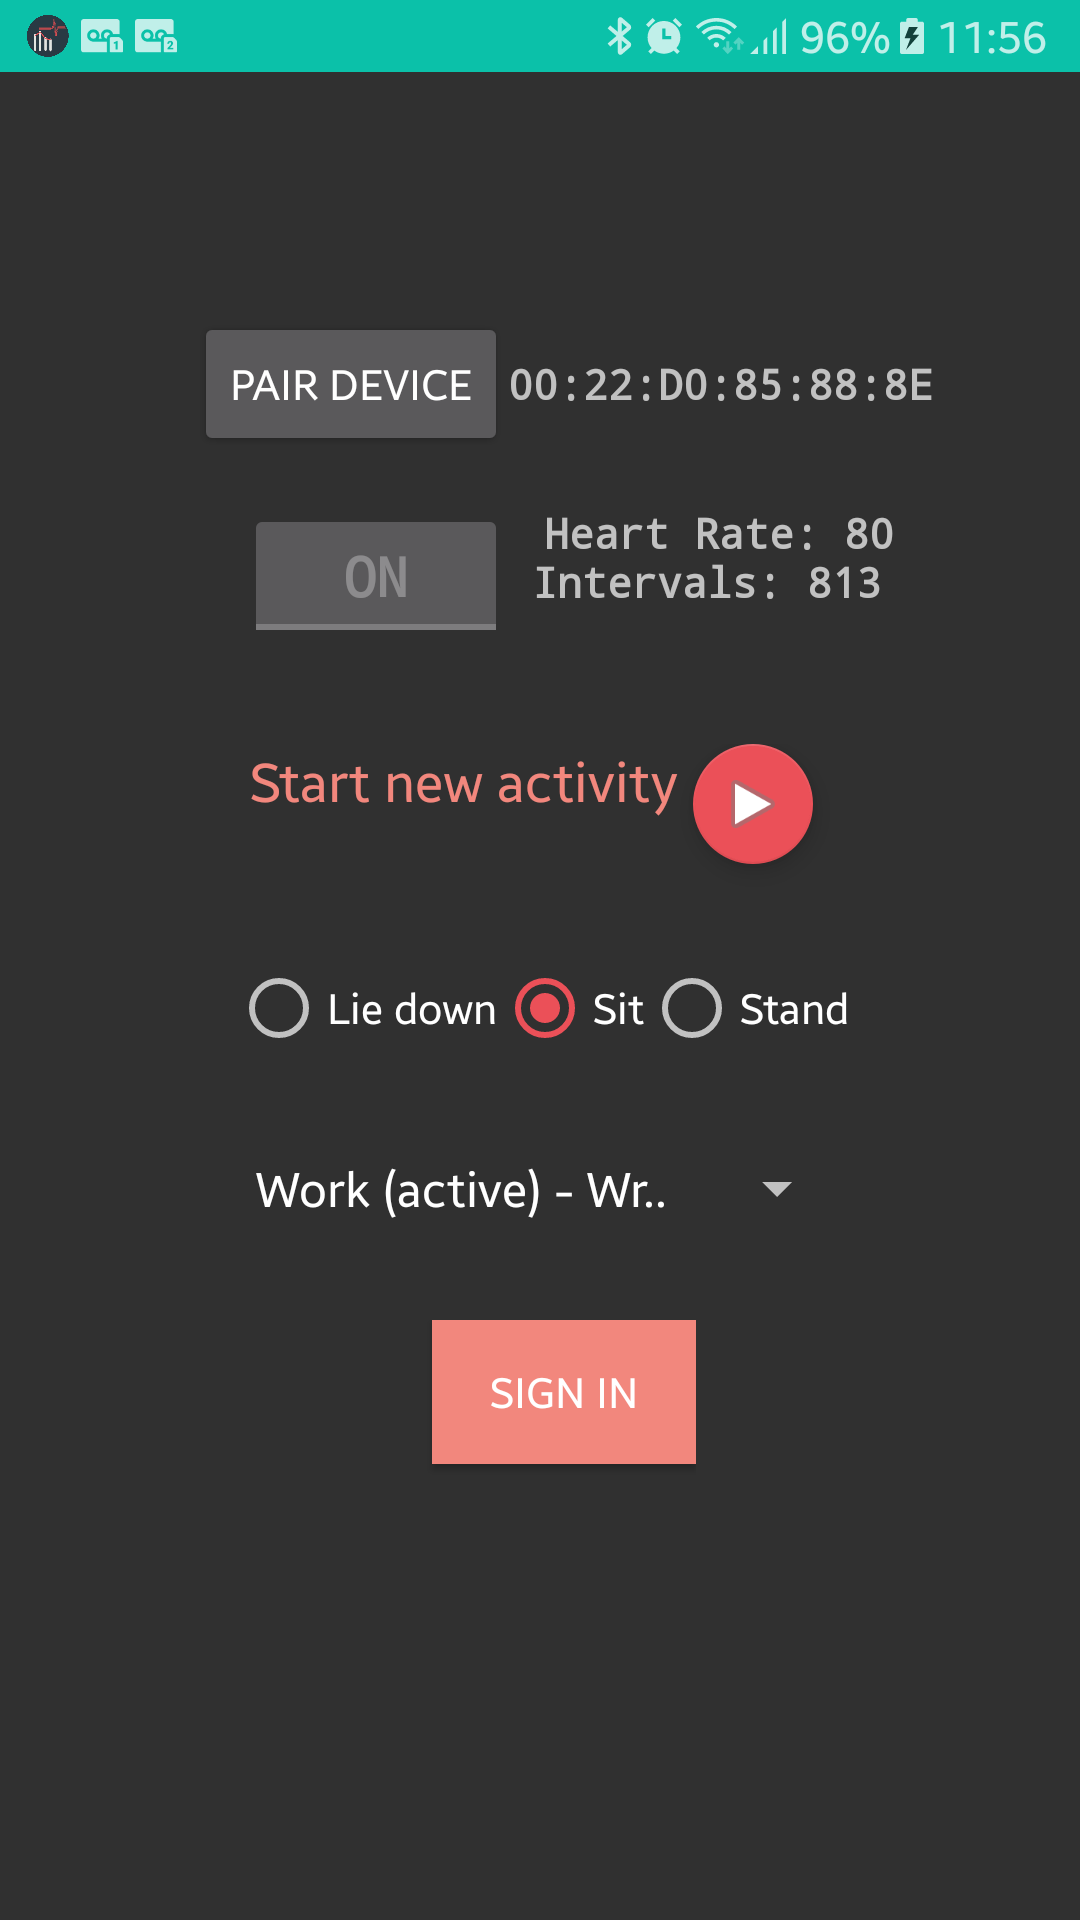
\includegraphics[width=0.33\textwidth]{apptela}
            	\caption{Captura de tela do aplicativo para coleta de dados com a informação do último intervalo recebido do sensor e a interface para o usuário registrar uma sessão de atividade}
                \label{apptela}
            \end{figure}
            
            \paragraph{} Está em andamento o desenvolvimento de uma interface onde serão disponibilizadas para o usuário as visualizações de seus dados, como a série de intervalos e evolução de suas métricas agregadas, além da possibilidade de editar as atividades registradas.
        
        \subsection{Categorização e registro de atividades} \label{categories}
    
            \paragraph{} Para que o usuário registrasse a atividade exercida, conforme interface mostrada na figura ~\ref{apptela}, foi desenvolvida, inicialmente, uma lista fixa de categorias de atividades. Caso contrário, o usuário poderia adicionar qualquer tipo de atividade, o que dificultaria ou até impossibilitaria a análise, visto que a tendência é que houvesse poucos exemplos de diversas atividades semelhantes. 
            
            \paragraph{} Entretanto, como essa lista foi criada preliminarmente para podermos iniciar a coleta, ainda não tínhamos como identificar quais tipos de atividades iríamos, de fato, poder distinguir. Sendo assim, essa lista está em constante modificação, através de um ciclo de \textit{feedback} com o resultado das análises exploratórias e dos classificadores. Conforme mais dados vão sendo adicionados, tentamos detalhar melhor a granularidade da lista, agrupando categorias ou criando novas. Contudo, a categorização das atividades já realizadas pelo usuário anteriormente mantém sua descrição original, e é mapeada para uma nova, se necessário, durante o pipeline.
            
            \paragraph{} Outros fatores influenciam as medições de HRV, tais como o consumo de cafeína ou álcool, a postura, a alimentação, o período do dia e alterações de humor. A postura já está sendo registrada no aplicativo e pretendemos incluir um campo de observações para poder registrar os outros fatores, mesmo que no formato de texto não estruturado, para que sejam disponibilizados para outros tipos de análise que possam fazer uso do aplicativo e do pipeline.
            

%%----------------------------------------------------------------------------------------------------------
%%      PIPELINE
%%-----------------------------------------------------------------------------------------------------------

    \section{Desenvolvimento do Pipeline}
    \label{Pipeline}
    
        \subsection{Pré-visualização}        
        
            \paragraph{} Através da simples observação do valor bruto dos intervalos coletados em 24h, é possível observar padrões distintos de flutuação nos valores, de acordo com as atividades diárias. Na figura ~\ref{raw_day}, é possível notar que os intervalos ficam consideravelmente mais altos e irregulares em períodos de descanso, como sono e relaxamento. Além disso, durante períodos de exercício ou estresse de trabalho, ficam mais baixos e regulares. 
        
            \begin{figure}[h!]
            	\centering
            	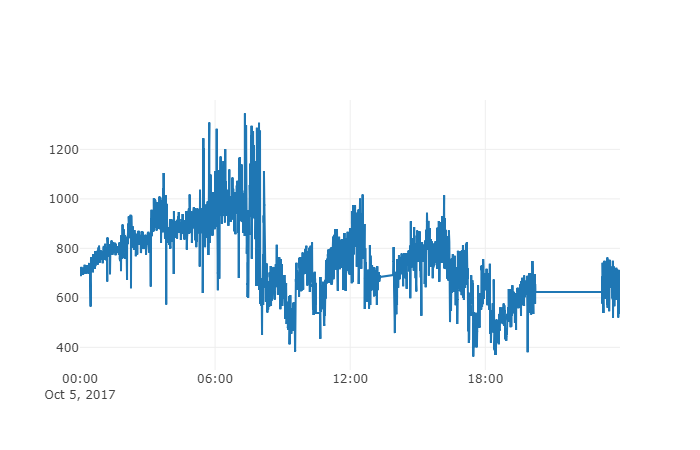
\includegraphics[width=0.7\textwidth]{raw_day}
            	\caption{Série temporal dos intervalos R-R registrados durante um dia. A série foi suavizada com uma média móvel de meia-janela de 15 pontos para facilitar a visualização. Os intervalos são mais espaçados e irregulares em situações de relaxamento como o sono, e mais curtos e regulares durante o movimento ou em situações de estresse}
                \label{raw_day}
            \end{figure}
        
        \subsection{Remoção de outliers e artefatos}
        
            \paragraph{} Apesar do posicionamento do coração garantir um sinal mais limpo do que o de um EEG, esse sinal não é, naturalmente, livre de ruídos e artefatos. Uma causa natural para a geração de ruído são os batimentos ectópicos, causados por condução elétrica originada em fibras fora do nó sinoatrial, região do músculo cardíaco responsável pelos impulsos elétricos que causam os batimentos regulares. Além disso, há a possibilidade de mal funcionamento no hardware do sensor, seja por falta de contato com a pele para detectar o impulso ou por falha no algoritmo interno de detecção do complexo QRS. 
            
            \paragraph{} Para remover esse tipo de ruído, aplicamos no dado um filtro para remoção de outliers que consiste em duas estratégias. A primeira é remover todos os intervalos com valores absolutos fora de um \textit{threshold}, que é configurável na execução do pipeline. Para as análises apresentadas nesse trabalho, consideramos aceitáveis os intervalos dentro do limite $300 <= RR <= 1800$. 
            
            \paragraph{} A segunda estratégia é baseada em uma média móvel que nos permite definir se um intervalo é um \textit{outlier} relativo ao contexto em que se encontra. Definimos como uma \textbf{sequência contínua} qualquer sequência de intervalos que não tenha um \textit{gap} maior que 3s entre seus \textit{timestamps}. Sempre que ocorre um \textit{gap} maior que esse valor entre dois intervalos consecutivos nos dados, uma sequência é quebrada no primeiro e outra iniciada no segundo intervalo. Para cada uma dessas sequências, passamos um filtro de média-móvel com meia-janela de tamanho 10 intervalos (total de 21 na janela) e, quando um intervalo está mais de 3 desvios-padrão acima ou abaixo da média da janela centrada nele próprio, ele é considerado um \textit{outlier} e removido.

            %%JUINCLUDEFIGURE comparação de um dado com e sem outlier/ectopic beat
        
        \subsection{Extração de sessões}
        
            \paragraph{} Até esse ponto, o pipeline trabalha com todos os intervalos disponíveis. Todavia, nem todos são usados na classificação de atividades, visto que o aplicativo permanece coletando-os enquanto o sensor estiver ativo, mesmo fora do tempo das atividades registradas pelo indivíduo. O próximo passo do pipeline é, portanto, extrair do banco de dados de intervalos apenas os que fazem parte de alguma atividade e agrupá-los com as informações das atividades registradas. Definimos esse conjunto de dados como \textbf{sessão}. Uma sessão é constituída por:
            
            \begin{itemize}
                \item O tipo da atividade exercida;
                \item O horário de início da sessão, para referência posterior;
                \item A duração total, calculada pelo final da atividade informada pelo indivíduo. Não necessariamente os intervalos registrados cobrem todo o período. É possível, por exemplo, que o sensor perca contato com o aparelho de celular com o qual estava conectado, interrompendo a sequência de intervalos antes do fim da atividade.
                \item Todos os intervalos do banco que estejam contidos no período entre o início e o fim da atividade;
            \end{itemize} 
            
            \paragraph{} A seleção dos intervalos que estão contidos em uma sessão é determinada pelo \textit{timestamp} dos eventos. Cabe ressaltar que o sensor apenas provê o valor em ms do intervalo, não contando com um \textit{timestamp}, que é adicionado no aplicativo de coleta, com frequência de 1Hz. Dessa forma, a referência que consta no intervalo armazenado no banco de dados é ao momento em que o intervalo foi recebido e não ao batimento propriamente. No entanto, como nossa análise é realizada sobre o comprimento dos intervalos e a relação entre intervalos consecutivos, isso não afeta nossa medição.
            
            %%JUINCLUDEFIGURE visualização de dois ou três tipos de sessão (histograma/time series)
            
            
        \subsection{Fragmentação} \label{fragdesc}
        
            \paragraph{} Conforme recomendações para a análise de HRV \cite{Quintana2016GuidelinesCommunication}, optamos por fragmentar cada sessão em segmentos de igual duração para que possam ser comparados dentro dos mesmos parâmetros. Caso contrário, haveria um desequilíbrio entre sessões de atividades cuja duração é muito diferente, por exemplo, uma sessão de sono de 8h e uma sessão de corrida de 15 minutos. Em geral, a análise de HRV é descrita como sendo de curta duração se tiver em torno de 5 minutos, e de ultra-curta duração se tiver menos tempo \cite{TaskForceoftheEuropeanSocietyofCardiologytheNorthAmericanSocietyofPacing1996HeartUse, Shaffer2017AnNorms.}.
            
            \paragraph{} O pipeline implementado permite a configuração da duração de cada fragmento. Além disso, é possível também configurar um período chamado de \textit{crop}, que é removido do início de cada sessão e não entra nos fragmentos, para suprimir o possível ruído causado pela adaptação da frequência cardíaca do indivíduo ao início da nova tarefa, também seguindo recomendações de análise \cite{Quintana2016GuidelinesCommunication}. 
            
            \paragraph{} Com esses dos parâmetros, são determinados o tempo de início e fim de cada fragmento dentro de uma sessão. Assim como na geração da sessão, os intervalos contidos em cada fragmento são determinados através da comparação de seu \textit{timestamp} com os horários de início e fim determinados para o fragmento.
            
        \subsection{Hierarquização de categorias}
        
            \paragraph{} Nesse passo do \textit{pipeline}, também é realizado o mapeamento de categorias de atividades que deixaram de ser utilizadas, conforme o ciclo de \textit{feedback} descrito na seção ~\ref{categories}, para que todas as atividades registradas estejam padronizadas para a entrada de treinamento dos classificadores. 
            
            \paragraph{} Uma das estratégias que adotamos é a de gerar múltiplas classes agregando categorias de em diferentes hierarquias para compará-las. Dessa forma, é possível selecionar uma lista de atividades disponíveis para incluir em uma supercategoria e incluir no dataset uma coluna com os labels de cada hierarquia. Além disso, incluímos também colunas para cada supercategoria de cada hierarquia, onde os valores são binários (o exemplo pertence ou não à categoria), para que possam ser testados tanto algoritmos de classificação binária quanto generalizações para múltiplas classes.
            
        \subsection{Cálculo das métricas agregadas}
        
            \paragraph{}A seguir, são calculadas as métricas agregadas da distribuição dos intervalos, conforme descritas na seção ~\ref{HRV}. Calculamos essas métricas para a distribuição dos intervalos tanto das sessões como dos fragmentos. Apesar de apenas os fragmentos serem utilizados nos classificadores, as métricas das sessões são úteis para análises de dados exploratórias, visualização e comparação das sessões por tipo de atividade. As métricas utilizadas são descritas na tabela ~\ref{feats}.
  
            \begin{table}[h!]
                \centering
                \begin{tabular}{ll}
                MRRI  & média dos valores dos intervalos                             \\
                SDNN  & desvio-padrão dos valores dos intervalos                     \\
                RMSSD & média RMS dos valores das diferenças entre dois intervalos consecutivos \\
                PNN50 & porcentagem dos intervalos consecutivos cuja diferença é superior a 50ms \\
                LFNU  & valor normalizado da potência do espectro na faixa 0.04–0.15Hz\\
                HFNU  & valor normalizado da potência do espectro na faixa 0.15–0.40Hz\\
                HF:LF & razão entre os valores de HF e LF
                \end{tabular}
                \caption{Métricas agregadas calculadas para cada fragmento e sessão e utilizadas na análise dos dados e classificação}
                \label{feats}
            \end{table}
            
            \paragraph{}Apesar de armazenados, valores como MHR (média de frequência cardíaca) e NN50 (número absoluto de intervalos consecutivos cuja diferença é superior a 50ms), LF e HF (valores absolutos da potência do espectro na baixa e alta frequências, em ms\textsuperscript{2}) não são utilizados nas análises, por serem diretamente correlacionados, respectivamente com o MRRI, PNN50, LFNU e HFNU, das quais derivam ou são derivados, sendo, portanto, redundantes. 
            
            \paragraph{} Além disso, a VLF (potência do espectro na faixa de 0.0003Hz a 0.04Hz) também é armazenada, mas não utilizada nas análises porque seu período (25s a 333s) elevado inviabiliza a presença de ciclos suficientes em dados de ultra-curta duração, sendo recomendado que não se utilize tal métrica, a não ser em análises de longa duração \cite{TaskForceoftheEuropeanSocietyofCardiologytheNorthAmericanSocietyofPacing1996HeartUse}.
        
           \paragraph{} Cada execução completa do pipeline, desde a remoção de artefatos até o cálculo das métricas, leva à geração de um \textit{dataset} para análise. A nomenclatura do \textit{dataset} gerado indica os parâmetros escolhidos para \textit{crop} e duração do fragmento. Para a geração desse \textit{dataset} são excluídas as listas de intervalos e mantidas apenas as métricas agregadas e dados do fragmento e de sua sessão relacionada. Cada linha, portanto, tem o seguinte conteúdo:
                \begin{itemize}
                    \item id do usuário;
                    \item descrição da atividade;
                    \item índice identificador da sessão;
                    \item índice da ordenação relativa do fragmento dentro da sessão (esse dado nos permite, por exemplo, normalizar análises usando apenas os primeiros minutos de cada sessão);
                    \item \textit{timestamp} do início do fragmento;
                    \item todas as métricas agregadas descritas acima, incluindo as que não são usadas nas classificações, mas podem ser visualizadas, num total de 12 métricas.
                \end{itemize}
                
            %%JUINCLUDEFIGURE exemplo de fragmento
            %%JUINCLUDEFIGURE diagrama do pipeline
        
%----------------------------------------------------------------------------------------
%	CLASSIFICATION
%----------------------------------------------------------------------------------------
        
        
    \section{Classificação supervisionada de atividades}
    \label{classif}
    
        \subsection{Análise exploratória}
            
            \paragraph{} Antes de iniciar a classificação, uma análise exploratória nos permite avaliar a viabilidade da ideia, assim como detectar potenciais problemas ou erros nos dados. 
            \paragraph{}As figuras ~\ref{sess_box_ronald} e ~\ref{sess_box_all} mostram como se comportam a distribuição de algumas métricas selecionadas através de todas as sessões gravadas. Na figura ~\ref{sess_box_ronald}, foi selecionado um indivíduo para demonstrar como as métricas variam entre atividades. É possível observar que atividades como exercício e sono se destacam bastante das outras, uma indicação de que são atividades facilmente identificáveis. Já a figura ~\ref{sess_box_ronald} representa uma agregação de todas as atividades, com exceção dessas três, por indivíduo, ressaltando que, apesar de haver semelhança, há um padrão levemente distinto para cada um deles, o que indica que uma classificação intra-usuário deva funcionar melhor do que uma inter-usuário. Apesar das figuras representarem apenas um subconjunto das métricas, as outras se comportam de maneira parecida.
      
      
            \begin{figure}[h!]
                \centering
                \subfigure{
                    \label{sb1a}                    
                    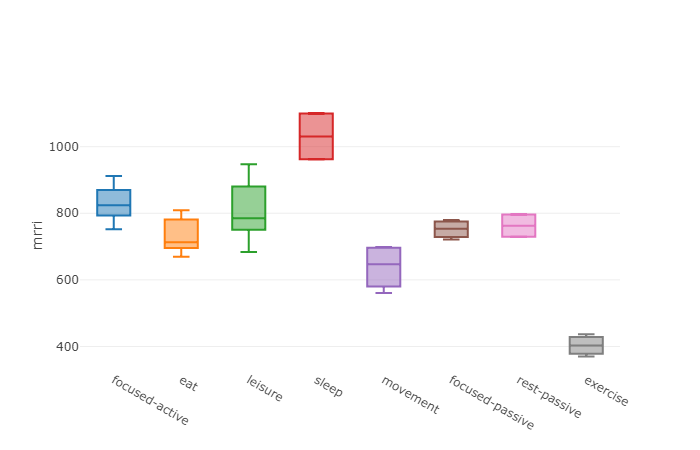
\includegraphics[width=0.75\textwidth]{sessions/sess_box_mrri_ronald.png}}
                \subfigure{
                    \label{sb1b}                    
                    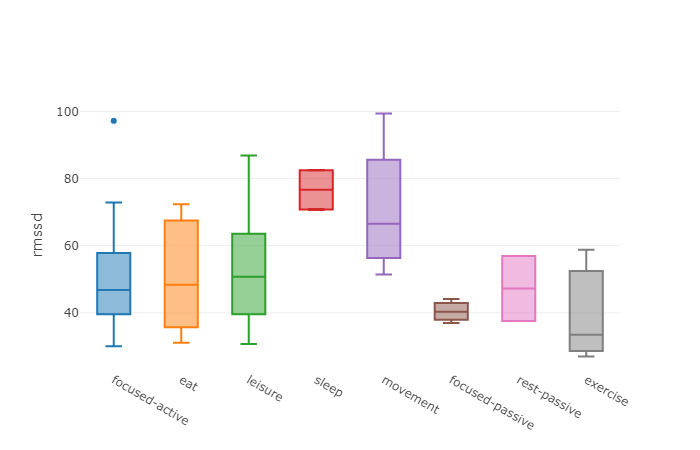
\includegraphics[width=0.75\textwidth]{sessions/sess_box_rmssd_ronald.png}}
                \caption{Distribuição da média dos intervalos e da média RMS da diferença entre intervalos consecutivos por sessão, para cada atividade. Apenas um indivíduo está representado.}
                \label{sess_box_ronald}
            \end{figure}

            \begin{figure}[h!]
                \centering
                \subfigure{
                    \label{sb2a}                    
                    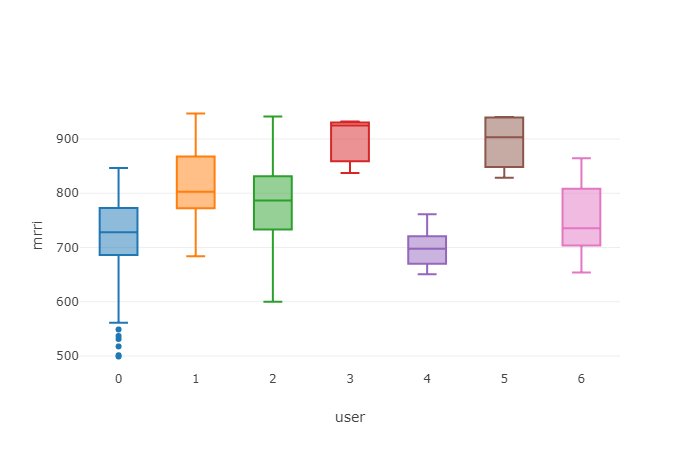
\includegraphics[width=0.75\textwidth]{sessions/sess_box_mrri_all.png}}
                \subfigure{
                    \label{sb2b}                    
                    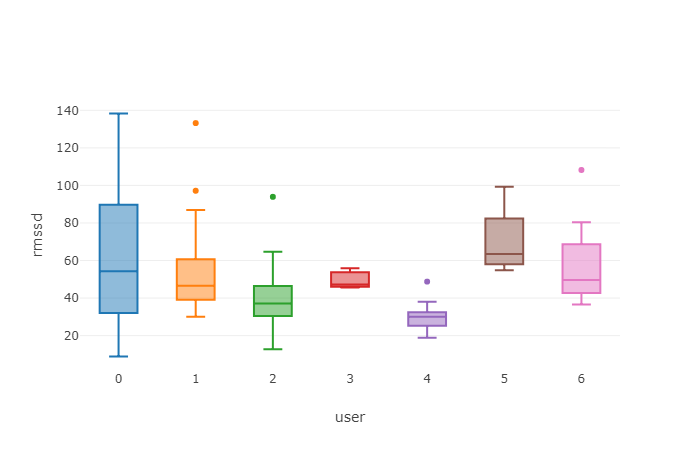
\includegraphics[width=0.75\textwidth]{sessions/sess_box_rmssd_all.png}}
                \caption{Distribuição da média dos intervalos e da média RMS da diferença entre intervalos consecutivos por sessão, para cada indivíduo. Foram agrupadas as sessões das diversas atividades, excluindo exercício, sono e movimento}
                \label{sess_box_all}
            \end{figure}

        \subsection{Preparação do dado}
        
            \paragraph{} No intuito de definir a configuração ótima dos parâmetros de duração do fragmento e \textit{crop} inicial, executamos o pipeline repetidamente, variando os valores desses dois parâmetros gerando um \textit{dataset} para cada par de parâmetros. Os valores testados foram (em segundos): 30, 60, 90 para o \textit{crop} e 60, 120, 180, 240, 300, 420, 600 para a duração.
        
            \paragraph{} Apesar do já termos executado a maior parte do tratamento necessário ao dado no pipeline de processamento, ainda foi necessária a normalização dos valores de cada \textit{feature}, realizada somente na fase do classificador. Para isso, cada \textit{dataset} é separado por indivíduo e, para cada um, é aplicada uma função que transforma cada uma das métricas em uma distribuição com média 0 e desvio-padrão 1. Isso impede que os classificadores atribuam um peso desproporcionalmente alto para \textit{features} que tenham alta variância.
            
            \paragraph{} Por fim, os datasets resultantes foram divididos em exemplos para treino e teste em uma proporção de 4:1. 
            
        \subsection{Métricas de avaliação da classificação}
            \paragraph{} Para avaliar o desempenho dos classificadores, usamos a métrica chamada de \textit{f1-score}, definida da seguinte forma:
            
            \paragraph{} Para cada classe resultante, sejam:
                \begin{itemize}
	                \item \textbf{tp} o número de verdadeiros positivos (exemplos corretamente identificados nessa classe);
	                \item \textbf{tn} o número de verdadeiros negativos (exemplos corretamente identificados como não pertencendo a essa classe);
	                \item \textbf{fn} o número de falsos negativos (exemplos que pertencem a essa classe, mas foram incorretamente classificados em outra);
	                \item \textbf{fp} o número de falsos positivos (exemplos que não pertecnem a essa classe, mas foram incorretamente classificados nela);
	                \item \textbf{Precisão} é a métrica definida como $\frac{tp}{tp + fp}$, representando a segurança em afirmar que um exemplo classificado realmente pertence a essa classe, ou seja, a habilidade de minimizar falsos positivos;
	                \item \textbf{Recall} é uma métrica definida como $\frac{tp}{tp + fn}$, representando a habilidade do classificador encontrar a maioria dos exemplos positivos, minimizando falsos negativos;
	                \item \textbf{F1-score}, por fim, é uma média ponderada da precisão e recall. É possível atribuir pesos diferentes para valorizar mais uma ou outra métrica, entretanto, nesse trabalho, vamos considerar seus pesos iguais. Logo, o f1-score pode ser escrito como $2 * \frac{precisao \cdot recall}{precisao + recall} $
                \end{itemize}
                
                \paragraph{} Nos resultados a seguir, a não ser que seja explicitamente definido de outra forma, estamos usando o f1-score para representar o desempenho das classificações.

        \subsection{Seleção de modelo}
        
            \paragraph{} Para a classificação, foram testados os algoritmos SVM com kernel linear e com kernel radial (RBF), e \textit{Random Forest}, por possuírem características desejáveis para o modelo propposto. O SVM, com o uso de kernels, permite trabalhar com dados de alta dimensionalidade e foi o primeiro algoritmo testado. No entanto, ele apresentou resultados abaixo do esperado, possivelmente por causa da grande variedade de classes testadas, quando a principal vantagem desse método é a separação binária. Por outro lado, o algoritmo \textit{Random Forest} é um método do tipo \textit{ensemble}, construído pela combinação de diversas classificações base independentes. Para cada métrica testada (\textit{feature}), o conjunto de treino é amostrado com reposição, o que reforça essa independência, sendo uma vantagem para as múltiplas classes. As implementações usadas para ambos os algoritmos foram do pacote \textit{scikit-learn} ~\cite{scikit}.
            
            \paragraph{} Os algoritmos foram executados usando \textit{5-fold cross-validation}, uma espécie de \textit{bootstrap} em que o \textit{dataset} de treino é dividido em 5 e, cada um dos sub-datasets resultantes é usado como validação uma vez, enquanto os outros quatro são usados para treino. Isso permite realizar a validação, mesmo com todos os exemplos sendo usados para treino. 
            
            \paragraph{} Para a seleção de modelo, fizemos uma avaliação do SVM em \textit{grid-search}, ou seja, variando seus parâmetros para verificar qual configuração oferece o melhor resultado. Para o kernel linear, o valor do parâmetro C, que reflete a regularização dos dados, deixando-os menos suscetíveis a ruídos, foi testado em um espaço de busca logarítmico de $10^{-3}$ até $10^{3}$. Para o kernel RBF, além desse mesmo parâmetro, o valor de $\gamma$, que reflete o raio de influência de um exemplo, foi testado no mesmo espaço de busca.
            
            \paragraph{} Nessa etapa de seleção de modelo, apresentamos o resultado apenas de um dataset, com fragmentos de comprimento 300s e \textit{crop} de 90s. Os resultados para outras configurações de fragmentação foram semelhantes. A tabela mostra, para cada classe, a comparação do resultado da melhor parametrização do SVM contra o \textit{Random Forest}. É possível observar que o \textit{ Random Forest} apresentou performance melhor que o SVM para todas as classes e, por isso, será utilizado nas próximas análises. 

        \subsection{Hierarquia}
        
        
\chapter{Discussão}
\label{Dicussion}

%Estudos Preliminares – Qual é o estado da arte na sua área de pesquisa?
%Questão-alvo - Qual é o problema que seu trabalho pretende atacar?
%Objetivos – O que o seu trabalho tenta alcançar?
%Significância – Por que o seu trabalho é importante?
%Metodologia - Como você pretende atacar este problema?

%----------------------------------------------------------------------------------------
%	CONTENT - APPENDICES
%----------------------------------------------------------------------------------------

\appendix % Cue to tell LaTeX that the following "chapters" are Appendices

% Include the appendices of the thesis as separate files from the Appendices folder
% Uncomment the lines as you write the Appendices

% Appendix A

\chapter{Cronograma Proposto para as Atividades Restantes} % Main appendix title

\label{AppendixA} % For referencing this appendix elsewhere, use \ref{AppendixA}

\paragraph{} Para concluir os objetivos do trabalho, propomos o seguinte cronograma para as atividades restantes:

\begin{itemize}
    \item Conclusão da migração do banco de dados - Maio/2018
    \item Conclusão da interface web para visualização dos intervalos e edição das atividades - Maio a Junho/2018
    \item Aplicação dos experimentos controlados - Junho a Agosto/2018
    \item Teste de novas técnicas de análise para melhorar o desempenho do classificador - Junho a Agosto/2018
    \item Implementação de interface para o treinamento com \textit{biofeedback} objetivando elevar ou reduzir o HRV voluntariamente - Junho/2018
    \item Coleta de dados do treinamento de \textit{biofeedback} - Junho a Agosto/2018
    \item Classificação em tempo real do HRV para implementação no protótipo de jogo como IHC - Agosto a Setembro/2018
    \item Conclusão do trabalho - Setembro/2018
\end{itemize}

%----------------------------------------------------------------------------------------
%	BIBLIOGRAPHY
%----------------------------------------------------------------------------------------

\printbibliography


%----------------------------------------------------------------------------------------

\end{document}  
